\begin{frame}
    \frametitle{Unterschied zwischen DHCP und einer statischen IP?}
    \framesubtitle{Im Hinblick auf den Energieverbrauch}

    \begin{columns}
        \begin{column}{0.5\textwidth}
            \begin{itemize}
                \item DHCP
                      \begin{itemize}
                          \item DHCP Server
                          \item Dynamische Zuweisung von IP Adressen
                          \item Lease time
                      \end{itemize}
            \end{itemize}
        \end{column}
        \begin{column}{0.5\textwidth}
            \begin{itemize}
                \item Statische IP-Adresse
                      \begin{itemize}
                          \item IP Adresse bleibt statisch
                          \item Vergewissern, dass Adresse verfügbar
                      \end{itemize}
            \end{itemize}
        \end{column}
    \end{columns}
\end{frame}

\begin{frame}
    \frametitle{DHCP}
    \begin{columns}
        \begin{column}{0.5\textwidth}
            \begin{itemize}
                \item 4 Schritte notwendig
                \item IP Adresse nur "geliehen"
                \item Lease time-Erneuerung

            \end{itemize}
        \end{column}
        \begin{column}{0.5\textwidth}
            \begin{figure}
                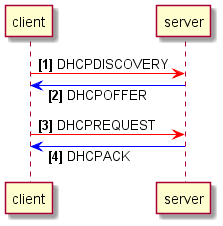
\includegraphics[scale=0.7]{../paper/fig/sequence_DHCP_connection.png}
            \end{figure}
        \end{column}
    \end{columns}
\end{frame}

\begin{frame}
    \frametitle{Experimentdurchlauf: DHCP}
    \begin{figure}
        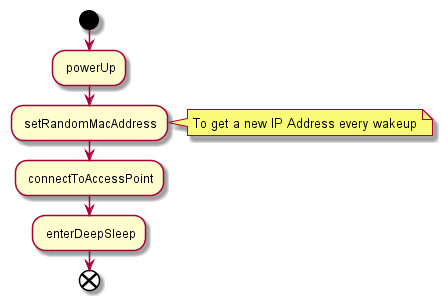
\includegraphics[scale=0.6]{../paper/fig/sequence_DHCP.png}
    \end{figure}
\end{frame}

\begin{frame}
    \frametitle{Experimentdurchlauf: Statische IP}
    \begin{figure}
        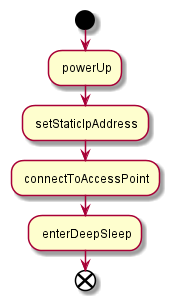
\includegraphics[scale=0.6]{../paper/fig/sequence_static_ip.png}
    \end{figure}
\end{frame}

\begin{frame}
    \frametitle{Messergebnisse: DHCP}
    \begin{columns}
        \begin{column}{0.35\textwidth}
            \begin{itemize}
                \item $\overline{Dauer}$: $\approx5.5s$
                \item $\overline{Verbrauch}$: $\approx0.35As$
            \end{itemize}
        \end{column}
        \begin{column}{0.65\textwidth}
            \begin{figure}
                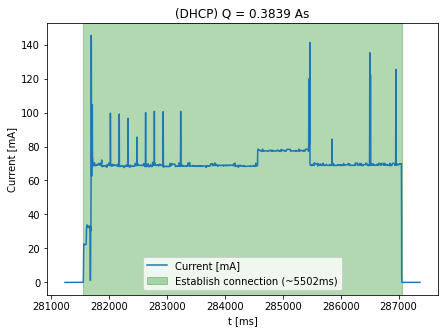
\includegraphics[scale=0.5]{../paper/fig/dhcp.png}
            \end{figure}
        \end{column}
    \end{columns}
\end{frame}

\begin{frame}
    \frametitle{Messergebnisse: Statische IP}
    \begin{columns}
        \begin{column}{0.35\textwidth}
            \begin{itemize}
                \item $\overline{Dauer}$: $\approx4.0s$
                \item $\overline{Verbrauch}$: $\approx0.28As$
            \end{itemize}
        \end{column}
        \begin{column}{0.65\textwidth}
            \begin{figure}
                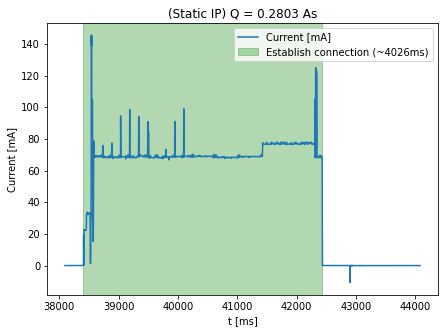
\includegraphics[scale=0.5]{../paper/fig/static_ip.png}
            \end{figure}
        \end{column}
    \end{columns}
\end{frame}

\begin{frame}
    \frametitle{Zusammenfassung}

    \begin{itemize}
        \item Verwenden einer statischen IP verbraucht $\approx 20.5\%$ weniger Strom
        \item Verbrauch beim Verwenden von DHCP abhängig von der Lease time
        \item Verbindungsaufbau über DHCP braucht $\approx 1.5s$ länger
    \end{itemize}


\end{frame}
